\documentclass{article}
\usepackage{amsmath}
\usepackage{graphicx}
\usepackage{tikz}
\usepackage{pgfplots}
\pgfplotsset{compat=1.18}
\usepackage{sectsty}

\sectionfont{\centering}

\title{CalcStudio Math Documentation}
\author{Aayush Koora}
\date{\today}

\begin{document}

\maketitle

\newpage
\section{Derivative: Tangent Line at Point}

\noindent
A derivative is the instantaneous rate of change of a function. It answers how fast a function is changing at a specific point \( x = a \).

\vspace{1em}

This is the formal definition of a limit:

\vspace{1em}

\begin{equation}
f'(a) = \lim_{h \to 0} \frac{f(a + h) - f(a)}{h}
\end{equation}

\vspace{1.5em}

\begin{center}
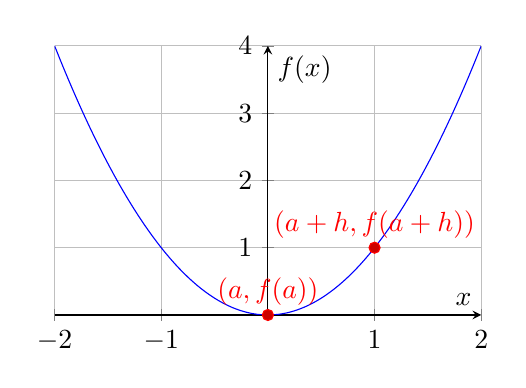
\begin{tikzpicture}
\begin{axis}[
    axis lines=center,
    xlabel=$x$,
    ylabel={$f(x)$},
    grid=both,
    width=7cm,
    height=5cm,
]
\addplot [
    domain=-2:2,
    samples=100,
    color=blue,
]
{x^2};
\addplot+[
    only marks,
    mark=*,
    nodes near coords,
    point meta=explicit symbolic,
] coordinates {
    (0, 0)[$(a, f(a))$]
    (1, 1)[$(a+h, f(a+h))$]
};
\end{axis}
\end{tikzpicture}
\end{center}

\vspace{1.5em}

\noindent
We can decrease \( h \) until it is infinitely small. As the distance between the two points (\( h \)) approaches 0, we get the instantaneous slope of \( f(x) \) at point \( a \).

\vspace{1em}

\noindent
A tangent line is a line that touches a function at one point and has the same slope as that instantaneous point.

\vspace{1em}

\noindent
We can model a tangent line like this:

\vspace{1em}

\begin{equation}
y = f(a) + f'(a)(x - a)
\end{equation}

\vspace{1em}

\begin{center}
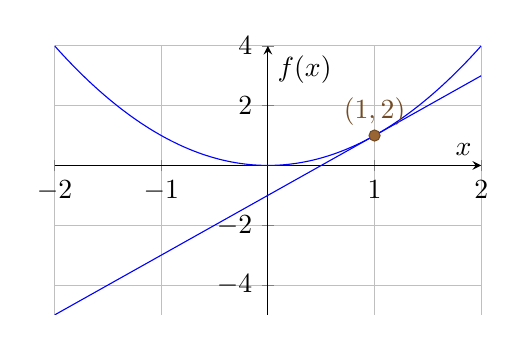
\begin{tikzpicture}
\begin{axis}[
    axis lines=center,
    xlabel=$x$,
    ylabel={$f(x)$},
    grid=both,
    width=7cm,
    height=5cm,
]
\addplot [
    domain=-2:2,
    samples=100,
    color=blue,
]
{x^2};
\addplot [
    domain=-2:2,
    samples=100,
    color=blue,
]
{2*x-1};
\addplot+[
    only marks,
    mark=*,
    nodes near coords,
    point meta=explicit symbolic,
] coordinates {
    (1, 1)[$(1, 2)$]
};
\end{axis}
\end{tikzpicture}
\end{center}

\newpage

\section{Integral: Area Under a Curve}

...coming soon...

\newpage

\section{Integral: Riemann Sum Approximation}

...coming soon...

\newpage

\section{Multivariable: Gradient Descent}

...coming soon...

\end{document}
